\vspace*{-5mm}
\mysection{Runtime View}
In this section we will see some Runtime Views in order to see how the components interact according to specific requests.\par
For the server-side we have taken into consideration the high-level Application Server only, without identifying the specific components of it. We also separate it from the DB, cause they are in 2 different machines.

\mysubsection{Event - Reserve Seat}
This Runtime View shows the different steps needed to reserve a seat. \par
We have to make an assumption : in the following diagram we reported only the most meaningful calls needed to achieve the goal. \par
So starting from the Main Activity the User can tap the “All Libraries” button and the EasyLib app will ask the server (and so the DB) to get the list of all of them. On return a new activity is started where thanks to a RecyclerView the list of all the libraries is displayed. \par
The user can next select the Library that he wants and like the libraries list, the information about this one are asked to the server and next displayed in the Book Activity. In this activity are displayed also the “library contents” (news, events and books), so user can select an event and automatically the EventActivity is opened and shown.\par
The app will check if there are available seats and if the user has already joined the event (in the diagram is called “checkEventStatus()”). So if there free seats and the event is not already joined then the “Reserve Seat” button is shown and the User can reserve a seat.
\newpage
\vspace*{0cm}
\begin{figure}[H]
	\centering
	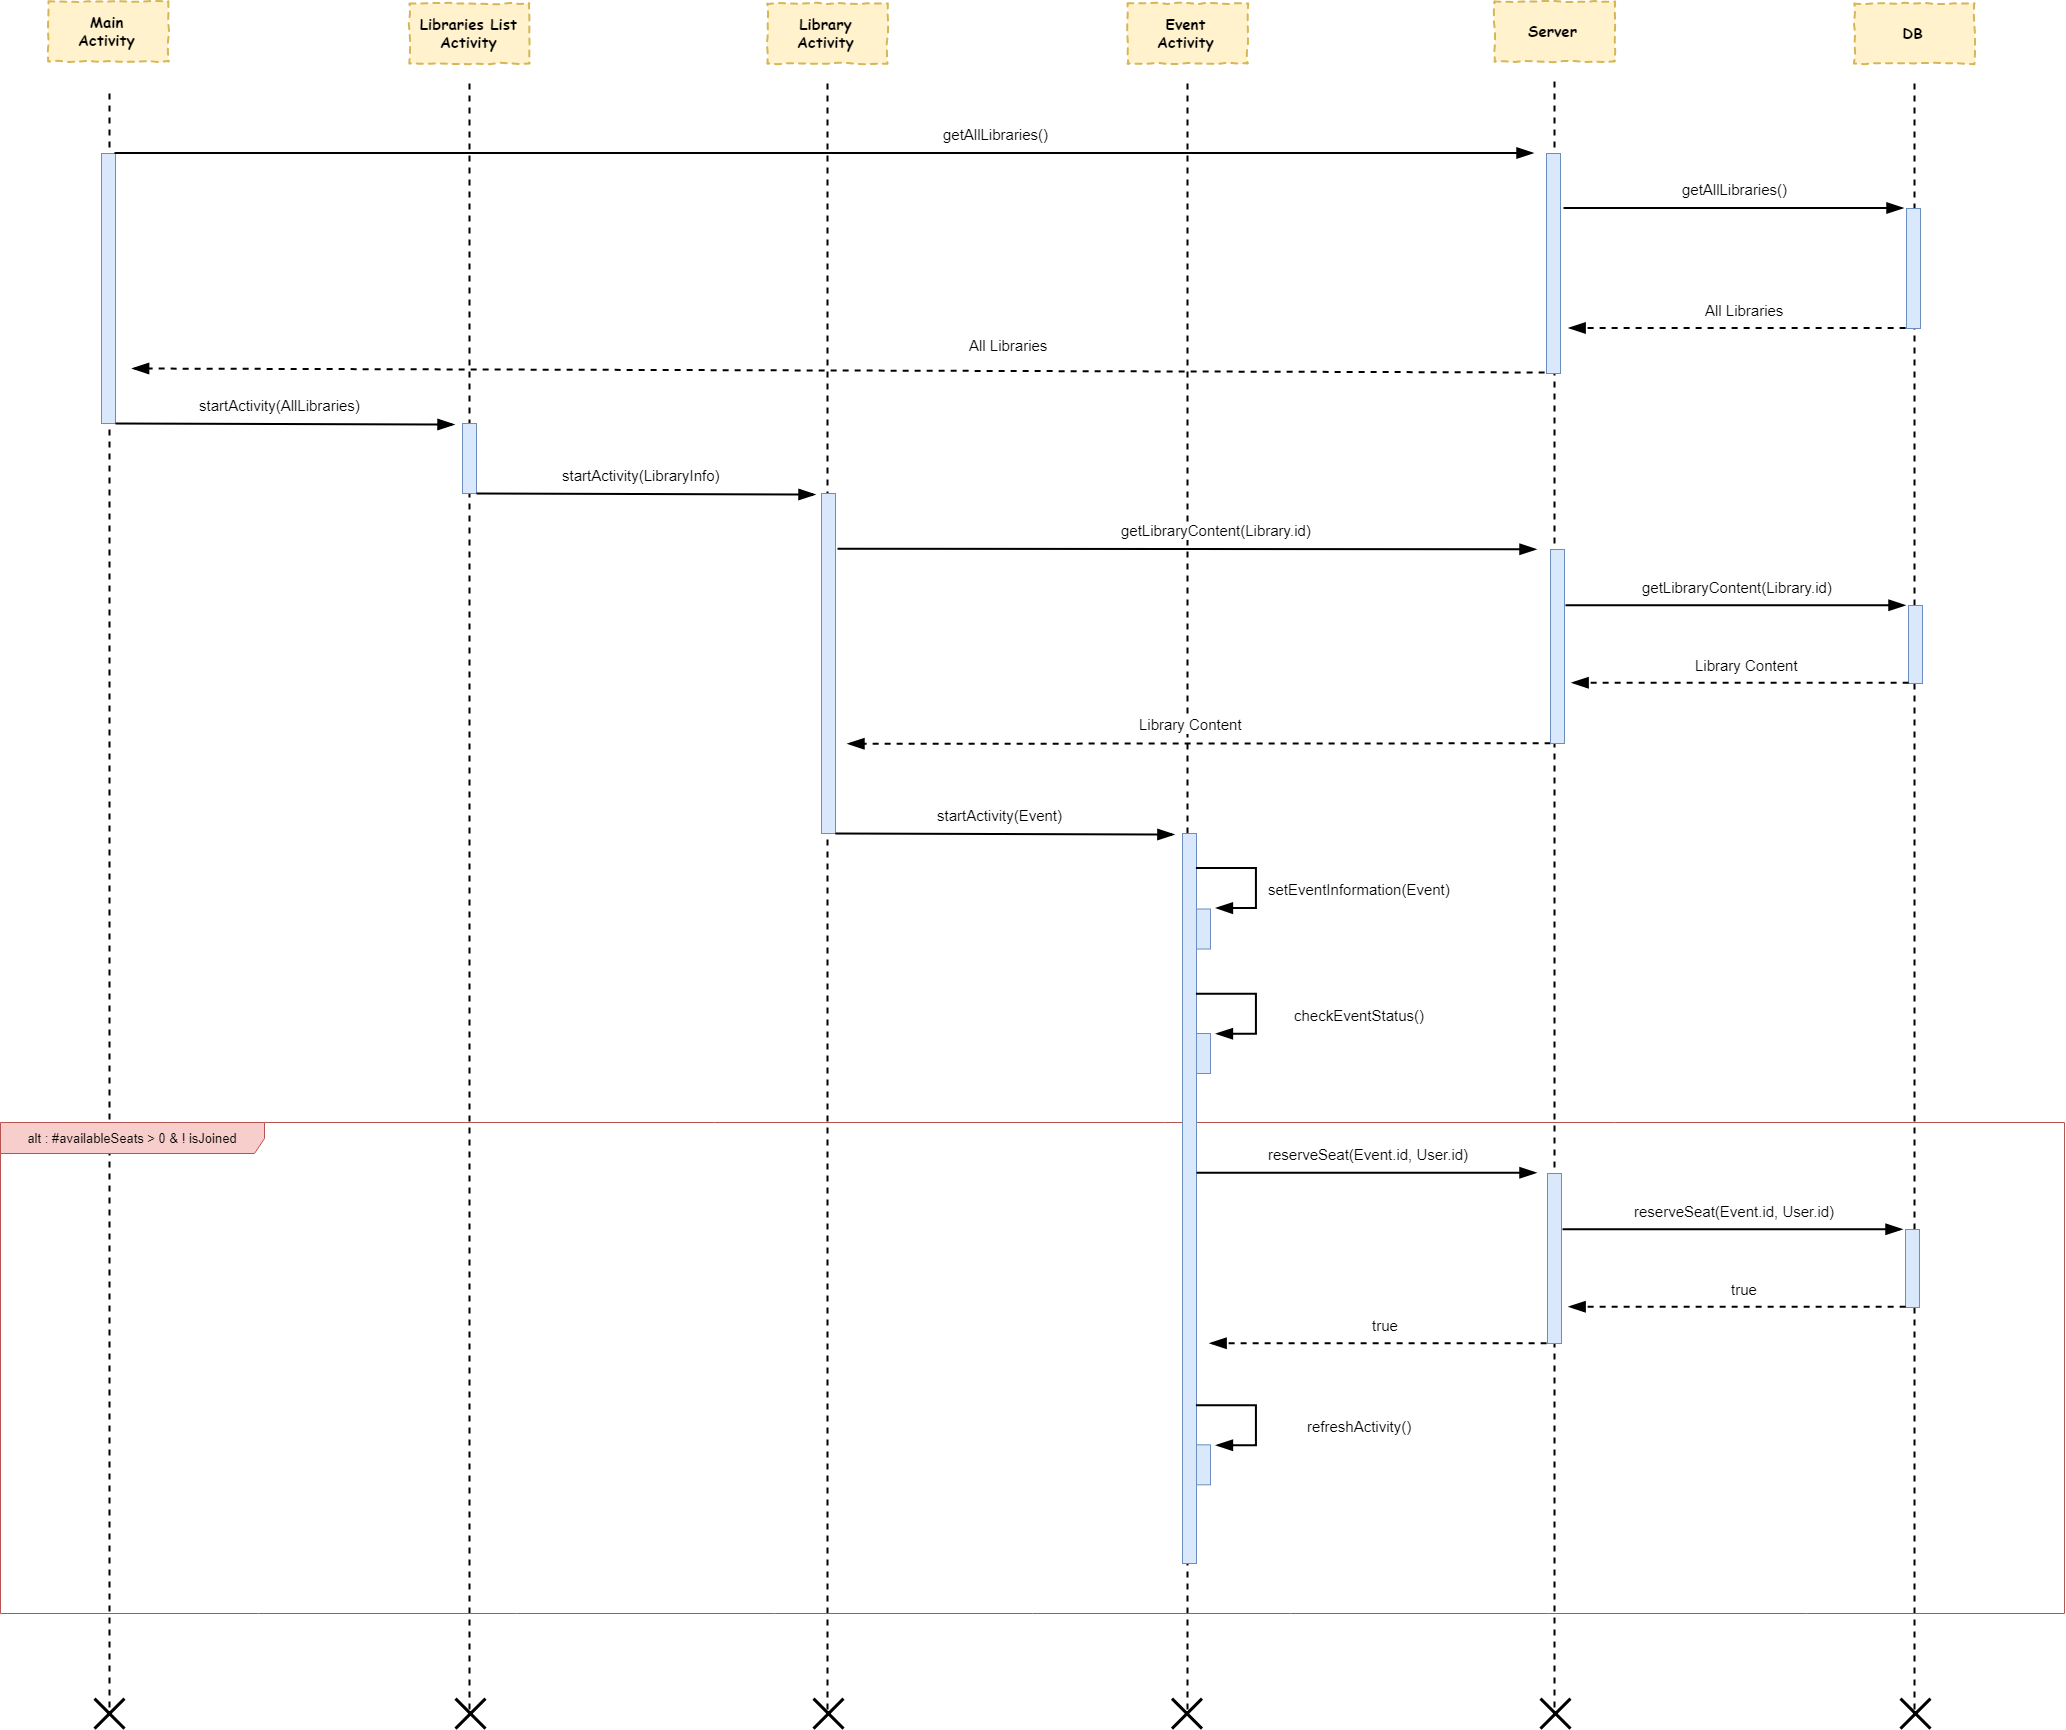
\includegraphics[scale=0.22]{Images/Runtime/event_reserve_seat}
	\caption{Event Reserve Seat - Runtime View}
\end{figure}